%%%%%%%%%%%%%%%%%%%%%%%%%%%%%%%%%%%%%%%%%
% Beamer Presentation
% LaTeX Template
% Version 1.0 (10/11/12)
%
% This template has been downloaded from:
% http://www.LaTeXTemplates.com
%
% License:
% CC BY-NC-SA 3.0 (http://creativecommons.org/licenses/by-nc-sa/3.0/)
%
%%%%%%%%%%%%%%%%%%%%%%%%%%%%%%%%%%%%%%%%%

%----------------------------------------------------------------------------------------
%	PACKAGES AND THEMES
%----------------------------------------------------------------------------------------

%-- coding: UTF-8 --
\documentclass[UTF8,mathserif]{beamer}

\mode<presentation> {

% The Beamer class comes with a number of default slide themes
% which change the colors and layouts of slides. Below this is a list
% of all the themes, uncomment each in turn to see what they look like.

%\usetheme{default}
%\usetheme{AnnArbor}
%\usetheme{Antibes}
%\usetheme{Bergen}
%\usetheme{Berkeley}
%\usetheme{Berlin}
%\usetheme{Boadilla}
%\usetheme{CambridgeUS}
%\usetheme{Copenhagen}
%\usetheme{Darmstadt}
%\usetheme{Dresden}
%\usetheme{Frankfurt}
%\usetheme{Goettingen}
\usetheme{Hannover}
%\usetheme{Ilmenau}
%\usetheme{JuanLesPins}
%\usetheme{Luebeck}
%\usetheme{Madrid}
%\usetheme{Malmoe}
%\usetheme{Marburg}
%\usetheme{Montpellier}
%\usetheme{PaloAlto}
%\usetheme{Pittsburgh}
%\usetheme{Rochester}
%\usetheme{Singapore}
%\usetheme{Szeged}
%\usetheme{Warsaw}

% As well as themes, the Beamer class has a number of color themes
% for any slide theme. Uncomment each of these in turn to see how it
% changes the colors of your current slide theme.

%\usecolortheme{albatross}
%\usecolortheme{beaver}
%\usecolortheme{beetle}
%\usecolortheme{crane}
%\usecolortheme{dolphin}
%\usecolortheme{dove}
%\usecolortheme{fly}
%\usecolortheme{lily}
%\usecolortheme{orchid}
%\usecolortheme{rose}
%\usecolortheme{seagull}
%\usecolortheme{seahorse}
%\usecolortheme{whale}
%\usecolortheme{wolverine}

%\setbeamertemplate{footline} % To remove the footer line in all slides uncomment this line
%\setbeamertemplate{footline}[page number] % To replace the footer line in all slides with a simple slide count uncomment this line

%\setbeamertemplate{navigation symbols}{} % To remove the navigation symbols from the bottom of all slides uncomment this line
}

\usepackage{graphicx} % Allows including images
\usepackage{booktabs} % Allows the use of \toprule, \midrule and \bottomrule in tables
\usepackage[UTF8]{ctex}

\usepackage{amsmath,amsthm}%数学公式|数学符号blablabla
\usepackage{amsfonts}%数学公式|数学符号blablabla
\usepackage{amssymb}%数学公式|数学符号blablabla
\usepackage{graphicx}%图片


\usepackage{indentfirst}%首行缩进
\setlength{\parindent}{2em}

%----------------------------------------------------------------------------------------
%	TITLE PAGE
%----------------------------------------------------------------------------------------

\title[Short title]{Algorithms for Non-negative Matrix Factorization } % The short title appears at the bottom of every slide, the full title is only on the title page

\author{李睿易} % Your name
\institute[UCAS] % Your institution as it will appear on the bottom of every slide, may be shorthand to save space
{
University of Chinese Academy of Sciences \\ % Your institution for the title page
2018E8013261056 \\
\medskip
\textit{ruiyilii@163.com} % Your email address
}
\date{\today} % Date, can be changed to a custom date

\begin{document}

\begin{frame}
\titlepage % Print the title page as the first slide
\end{frame}

\begin{frame}
\frametitle{Overview} % Table of contents slide, comment this block out to remove it
\tableofcontents % Throughout your presentation, if you choose to use \section{} and \subsection{} commands, these will automatically be printed on this slide as an overview of your presentation
\end{frame}

%----------------------------------------------------------------------------------------
%	PRESENTATION SLIDES
%----------------------------------------------------------------------------------------

%------------------------------------------------
\section{背景介绍}
%------------------------------------------------

\subsection{背景}

\begin{frame}
    \frametitle{矩阵分解的意义}
    \begin{itemize}
      \item 海量数据对应的矩阵信息分布不均匀,对其进行计算效率低下,希望找到一种方法可以对矩阵信息进行压缩,提高计算效率。
      \item 大型矩阵分析难度大,对其进行分解,希望可以反应出矩阵的秩,特征值和奇异值等。
      \item 高维空间数据的稀疏性,希望对矩阵进行降维,压缩无意义数据。
    \end{itemize}
\end{frame}

\begin{frame}
    \frametitle{相关工作介绍}
    \begin{itemize}
        \item 主成分分析(Principal Component Analysis,PCA), 是一种统计方法。通过正交变换将一组可能存在相关性的变量转换为一组线性不相关的变量,转换后的这组变量叫主成分。
        \item K-means算法的基本思想是:以空间中k个点为形心进行聚类,对最靠近他们的对象归类。通过迭代的方法,逐次更新各簇的形心的值,直至得到最好的聚类结果。
    \end{itemize}
\end{frame}


\subsection{问题}

\begin{frame}
    \frametitle{问题}
    \begin{itemize}
        \item 存在问题:\\
            \quad \quad 虽然前述算法都可以执行矩阵分解,但是对数值并没有强约束,有可能在分解的矩阵中得到负值,虽然可以满足矩阵分解的要求,但是在实际生活中负值并没有任何意义,比如对图像进行分解,那么便无法理解出现的负值。
        \item 提出问题:\\
            \quad \quad 1、将原始矩阵进行分解,使得$V=WH$。\\
            \quad \quad 2、对分解的矩阵进行非负约束。
    \end{itemize}
\end{frame}



%------------------------------------------------
\section{算法介绍}
%------------------------------------------------

\subsection{算法简介}

\begin{frame}
\frametitle{代价函数}
    \begin{itemize}
        \item Euclidean distance:\\
            $$\|A-B\|^{2}=\sum_{ij}(A_{ij}-B_{ij})^{2}$$
        \item  "divergence" of A from B:\\
            $$D(A\|B)=\sum_{ij}(A_{ij}\log\frac{A_{ij}}{B_{ij}}-A_{ij}+B_{ij})$$
    \end{itemize}
\end{frame}


\begin{frame}
\frametitle{乘法因子}
    \indent 提出了乘法更新规则,不仅可以兼顾非负的约束,而且可以高效的对矩阵分解进行计算。\\
    \indent 通过以下更新规则可以保证Euclidean distance在每一次更新的时候都可以下降。 \\
    \begin{itemize}
        \item $H_{au}$\\
            $$H_{au}\leftarrow H_{au}\frac{(W^{T}V)_{au}}{(W^{T}WH)_{au}}$$
        \item $W_{ia}$\\
            $$W_{ia}\leftarrow W_{ia}\frac{V(H^{T})_{ia}}{WH(H^{T})_{ia}}$$
    \end{itemize}
\end{frame}


\begin{frame}
\frametitle{乘法因子}
    \indent 对于divergence有以下规则。同样可以证明在该更新规则下可以保证divergence距离每次更新都可以减小。\\
    \begin{itemize}
        \item $H_{au}$\\
            $$H_{au}\leftarrow H_{au}\frac{\sum_{i}W_{ia}V_{iu}/(WH)_{iu}}{\sum_{k}W_{ka}}$$
        \item $W_{ia}$\\
            $$W_{ia}\leftarrow W_{ia}\frac{\sum_{u}H_{au}V_{iu}/(WH)_{iu}}{\sum_{v}H_{av}}$$
    \end{itemize}
\end{frame}

\subsection{推导}

\begin{frame}
\frametitle{乘法因子的推导}
    \indent 接下来以Euclidean distance的推导为例进行推导,从噪声的分布和梯度下降来理解公式的推导。\\
    \indent 我们假设原始矩阵的噪声服从正态分布(divergence距离可以由服从泊松分布推得),则其最大似然函数为:\\
    \begin{equation}
    	L(W,H)=\prod\frac{1}{\sqrt{2\pi}\sigma_{ij}}exp(-\frac{(V_{ij}-(WH)_{ij})^{2}}{2\sigma_{ij}})
    \end{equation}
    \indent 对两边取对数可得:\\
    \begin{equation}
        \ln{L(W,H)}=\sum_{ij}\ln{\frac{1}{\sqrt{2\pi}\sigma_{ij}}}-\frac{1}{\sigma_{ij}}\frac{1}{2}\sum_{ij}[V_{ij}-(WH)_{ij}]^{2}
    \end{equation}
\end{frame}



\begin{frame}
\frametitle{乘法因子的推导}
    \indent 假设噪声的各方差一样为了使得上述函数取得最大值,只要保证下面的目标函数取最小:\\
    \begin{equation}
        l=\frac{1}{2}\sum_{ij}[V_{ij}-(WH)_{ij}]^{2}
    \end{equation}
    \indent 那么我们可以求得偏导:\\
    \begin{equation}
        \begin{split}
           \frac{\partial{l}}{\partial{H_{uj}}} & = \sum_{i}\sum_{j}(V_{ij}-\sum_{u}W_{iu}H_{uj})*(-W_{iu})\\
             & = -\sum_{i}W_{iu}*(V_{ij}-\sum_{u}W_{iu}H_{uj})\\
             & = -[(W^{T}V)_{uj}-(W^{T}WH)_{uj}]
        \end{split}
    \end{equation}
\end{frame}

\begin{frame}
\frametitle{乘法因子的推导}
    \indent 通过梯度下降算法,我们有:\\
    \begin{equation}
        \theta\leftarrow\theta-\alpha\nabla_{\theta}L(\theta)
    \end{equation}
    \begin{equation}
        H_{au}\leftarrow H_{au}+\eta_{au}[(W^{T}V)_{au}-(W^{T}WH)_{au}]
    \end{equation}
    \indent 如果我们选取$\eta_{au}=\frac{H_{au}}{(W^{T}WH)_{au}}$就可以将加减法操作变成乘法操作,称为乘法因子,得到以下迭代公式:\\
    \begin{equation}
        H_{au}\leftarrow H_{au}\frac{(W^{T}V)_{au}}{(W^{T}WH)_{au}}
    \end{equation}
    \indent 同理,我们可以推出来其余的三个迭代公式。
\end{frame}


%------------------------------------------------
\section{实验}
%------------------------------------------------

\subsection{算法实现}

\begin{frame}
\frametitle{NMF算法实验结果}
\begin{columns}[c] % The "c" option specifies centered vertical alignment while the "t" option is used for top vertical alignment
	
	\column{.45\textwidth} % Left column and width
	\textbf{乘法因子异步更新}
	\begin{enumerate}
		\item EucDis为Euclidean Distance代价函数值。
		\item DivDis为Divergence Distance代价函数值。
		\item 经过多次实验,DivDis收敛到稳定值的速度略优于EucDis。
	\end{enumerate}
	\column{.5\textwidth} % Right column and width
	\begin{figure}[h]%%图
		\centering  %插入的图片居中表示
		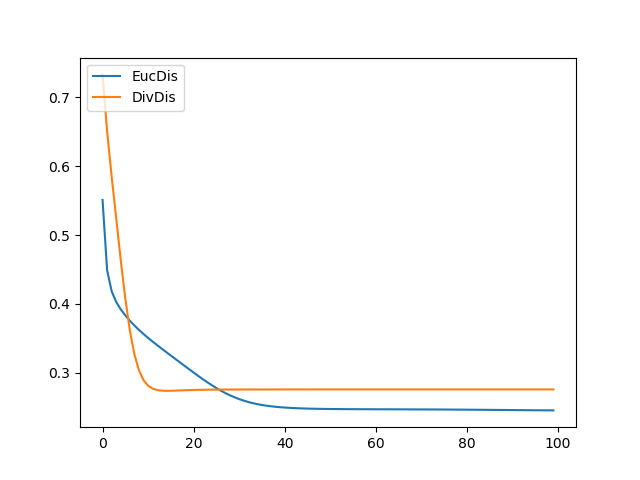
\includegraphics[width=1.2\linewidth]{image/Correct_answer}  %插入的图,包括JPG,PNG,PDF,EPS等,放在源文件目录下
		\caption{损失函数变化}  %图片的名称
		\label{fig:mcmthesis-logo}   %标签,用作引用
	\end{figure}
	
\end{columns}
\end{frame}


\begin{frame}
\frametitle{NMF算法实验结果}
\begin{columns}[c] % The "c" option specifies centered vertical alignment while the "t" option is used for top vertical alignment
	
	\column{.45\textwidth} % Left column and width
	\textbf{乘法因子同步更新}
	\begin{enumerate}
		\item 在实现代码的时候发现,乘法因子同步更新的正确性不能保证,结果如右图所示。
		\item 这是因为目标函数不是严格凸函数,此时找不到极值点。
	\end{enumerate}
	
	\column{.5\textwidth} % Right column and width
	\begin{figure}[h]%%图
		\centering  %插入的图片居中表示
		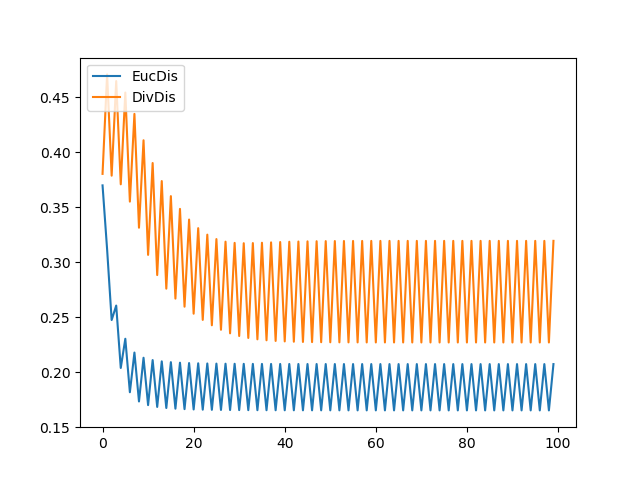
\includegraphics[width=1.2\linewidth]{image/Fail_answer}  %插入的图,包括JPG,PNG,PDF,EPS等,放在源文件目录下
		\caption{同步更新}  %图片的名称
		\label{fig:mcmthesis-logo}   %标签,用作引用
	\end{figure}
	
	
\end{columns}
\end{frame}


\begin{frame}
\frametitle{NMF算法的改进}
\indent 通过上面的实验结果可以看到,虽然NMF算法很巧妙的用乘法因子保证了结果为非负的约束,但是其收敛速度过慢。而且虽然该算法可以证明损失函数单调下降,但是并不一定可以找到一个稳定的收敛点,因此有以下几种改进算法。
\begin{itemize}
	\item Hoyer提出的带有稀疏性约束的NMF算法 
	\item Shahnaz提出的最小二乘约束下的梯度下降算法
	\item 由Paatero和Tapper提出的交替非负最小二乘法
	\item Lin提出的梯度投影法改进的NMF算法
	\item Cichoki等人提出的坐标轴下降更新算法
\end{itemize}
\end{frame}


%------------------------------------------------

\subsection{对比试验}


\begin{frame}
\frametitle{NMF算法}

\begin{columns}[c] % The "c" option specifies centered vertical alignment while the "t" option is used for top vertical alignment
	
	\column{.45\textwidth} % Left column and width
	\textbf{NMF}
	\begin{enumerate}
		\item 右图原图像在NMF算法中r在20到60的结果。
		\item 在达到稳定点后,r值越高,还原程度越好。
	\end{enumerate}
	
	\column{.5\textwidth} % Right column and width
	\begin{figure}[h]%%图
		\centering  %插入的图片居中表示
		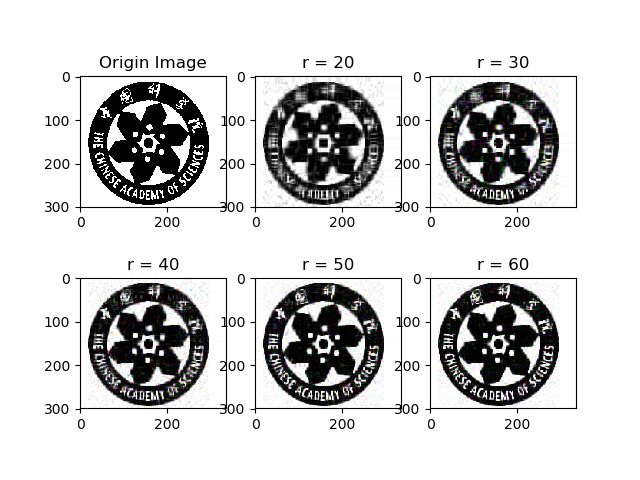
\includegraphics[width=1.2\linewidth]{image/Analyse_NMF}  %插入的图,包括JPG,PNG,PDF,EPS等,放在源文件目录下
		\caption{NMF}  %图片的名称
		\label{fig:mcmthesis-logo}   %标签,用作引用
	\end{figure}
	
	
\end{columns}
\end{frame}


\begin{frame}
\frametitle{PCA算法}

\begin{columns}[c] % The "c" option specifies centered vertical alignment while the "t" option is used for top vertical alignment
	
	\column{.45\textwidth} % Left column and width
	\textbf{PCA}
	\begin{enumerate}
		\item 右图为原图像在PCA算法中r在20到60的结果。
		\item 与NMF相比,达到稳定值之后图像会有一定的偏差,直观的感觉图像处理后会有黑边。
	\end{enumerate}
	
	\column{.5\textwidth} % Right column and width
	\begin{figure}[h]%%图
		\centering  %插入的图片居中表示
		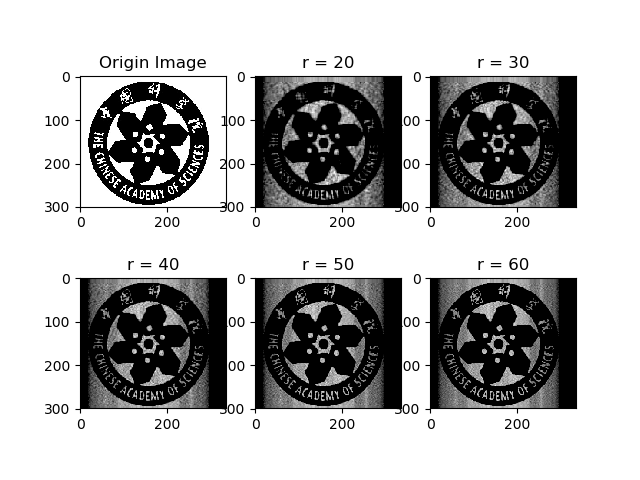
\includegraphics[width=1.2\linewidth]{image/Analyse_PCA}  %插入的图,包括JPG,PNG,PDF,EPS等,放在源文件目录下
		\caption{PCA}  %图片的名称
		\label{fig:mcmthesis-logo}   %标签,用作引用
	\end{figure}
	
	
\end{columns}
\end{frame}



\begin{frame}
\frametitle{Kmeans算法}

\begin{columns}[c] % The "c" option specifies centered vertical alignment while the "t" option is used for top vertical alignment
	
	\column{.45\textwidth} % Left column and width
	\textbf{Kmeans}
	\begin{enumerate}
		\item 右图为原图像在Kmeans算法中cluster在2到6的结果。
		\item 跟聚类点的个数关系不大,达到稳定值的时候都可以还原出高度近似的图像。
	\end{enumerate}
	
	\column{.5\textwidth} % Right column and width
	\begin{figure}[h]%%图
		\centering  %插入的图片居中表示
		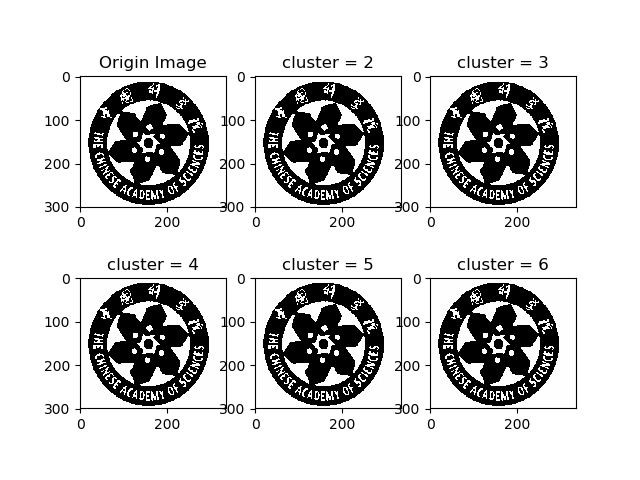
\includegraphics[width=1.2\linewidth]{image/Analyse_Kmeans}  %插入的图,包括JPG,PNG,PDF,EPS等,放在源文件目录下
		\caption{Kmeans}  %图片的名称
		\label{fig:mcmthesis-logo}   %标签,用作引用
	\end{figure}
	
	
\end{columns}
\end{frame}


%------------------------------------------------
\section{总结}
%------------------------------------------------

\subsection{总结}

\begin{frame}
\frametitle{总结}
\indent 对NMF的乘法因子进行了推导,并对原始NMF算法存在的问题进行了探讨,对几种矩阵分解方法(PCA,Kmeans)进行了对比验证,分析几种算法不同的作用。
\end{frame}

\subsection{引用}

\begin{frame}
\frametitle{引用}

\begin{itemize}
	\item Latex模板:\\
		\url{http://www.LaTeXTemplates.com}
	\item 代码及文档源文件:\\
		\url{https://github.com/AresDemmo/Algorithm/tree/master/Net_Data_Mining_Task_Reading}
\end{itemize}

\footnotesize{
\begin{thebibliography}{99} % Beamer does not support BibTeX so references must be inserted manually as below
	\bibitem[Lee and Seung, 2000]{p1} Daniel D. Lee and H. Sebastian Seung (2000)
	\newblock Algorithms for Non-negative Matrix Factorizatio
	\newblock \emph{NIPS 2000}.
\end{thebibliography}
}
\end{frame}

%------------------------------------------------

\begin{frame}
\Huge{\centerline{谢谢!}}
\end{frame}

%----------------------------------------------------------------------------------------

\end{document} 